\documentclass{article}

  % packages
    % basic stuff for rendering math
    \usepackage[letterpaper, top=1in, bottom=1in, left=1in, right=1in]{geometry}
    \usepackage[english]{babel}
    \usepackage{amsmath, amssymb} 
    \usepackage{bbm}              % for mathbbm

    % extra math symbols and utilities
    \usepackage{mathtools}        % for extra stuff like \coloneqq
    \usepackage{mathrsfs}         % for extra stuff like \mathsrc{}
    \usepackage{centernot}        % for the centernot arrow 
    \usepackage{bm}               % for better boldsymbol/mathbf 
    \usepackage{enumitem}         % better control over enumerate, itemize
    \usepackage{xr-hyper}	  % for external links
    \usepackage{hyperref}         % for hypertext linking
    \usepackage{fancyvrb}         % for better verbatim environments
    \usepackage{newverbs}         % for texttt{}
    \usepackage{xcolor}           % for colored text 
    \usepackage{listings}         % to include code
    \usepackage{lstautogobble}    % helper package for code
    \usepackage{parcolumns}       % for side by side columns for two column code
    \usepackage{algorithm} 	  % for algorithm pseudocode
    \usepackage{algpseudocode}	  % for algorithm pseudocode
    

    % page layout
    \usepackage{fancyhdr}         % for headers and footers 
    \usepackage{lastpage}         % to include last page number in footer 
    \usepackage{parskip}          % for no indentation and space between paragraphs    
    \usepackage[T1]{fontenc}      % to include \textbackslash
    \usepackage{footnote}
    \usepackage{etoolbox}

    % for custom environments
    \usepackage{tcolorbox}        % for better colored boxes in custom environments
    \tcbuselibrary{breakable}     % to allow tcolorboxes to break across pages

    % figures and tables 
    \usepackage{pgfplots}
    \pgfplotsset{compat=1.18}
    \usepackage{float}            % for [H] figure placement
    \usepackage{tikz, tikz-cd}
    \usetikzlibrary{arrows, positioning, calc}
    \usepackage{graphicx}
    \usepackage{caption, subcaption} 
    \usepackage{dcolumn}

    \usepackage[nottoc]{tocbibind}
    \hfuzz=5.002pt                % ignore overfull hbox badness warnings below this limit

  % New and replaced operators
    \DeclareMathOperator{\std}{std}
    \DeclareMathOperator*{\argmin}{\arg\!\min}
    \DeclareMathOperator*{\argmax}{\arg\!\max}
    \newcommand{\ket}[1]{\ensuremath{\left|#1\right\rangle}}
    \newcommand{\bra}[1]{\ensuremath{\left\langle#1\right|}}
    \newcommand{\braket}[2]{\langle #1 | #2 \rangle}
    \newcommand{\qed}{$\blacksquare \quad$}     % I like QED squares to be black

  % Custom Environments
    \tcbset{
      colframe = black,
      colback  = white,
      coltitle = black,
      colbacktitle = black!10,
      breakable, 
      arc=0mm,
      boxrule=1pt,
      left=8pt,
      right=8pt,
      top=6pt,
      bottom=6pt,
      before skip=12pt,
      after skip=12pt,
      bottomrule at break=-1pt,
      toprule at break=-1pt,
      fonttitle=\bfseries,
    }
    \newcounter{question}[section]
    \renewcommand{\thequestion}{\thesection.\arabic{question}}
    \NewDocumentEnvironment{question}{O{} o}{%
      \refstepcounter{question}%
      \ifstrempty{#1}{%
        \begin{tcolorbox}[title=\textbf{Question \thequestion}]%
      }{%
        \IfValueTF{#2}{%
          \begin{tcolorbox}[title=\textbf{Question \thequestion~(#1)}, label={#2}]%
        }{%
          \begin{tcolorbox}[title=\textbf{Question \thequestion~(#1)}]%
        }%
      }%
    }{%
      \end{tcolorbox}%
    }

    \newcounter{exercise}[section]
    \renewcommand{\theexercise}{\thesection.\arabic{exercise}}
    \NewDocumentEnvironment{exercise}{O{} o}{%
      \refstepcounter{exercise}%
      \ifstrempty{#1}{%
        \begin{tcolorbox}[title=\textbf{Exercise \theexercise}]%
      }{%
        \IfValueTF{#2}{%
          \begin{tcolorbox}[title=\textbf{Exercise \theexercise~(#1)}, label={#2}]%
        }{%
          \begin{tcolorbox}[title=\textbf{Exercise \theexercise~(#1)}]%
        }%
      }%
    }{%
      \end{tcolorbox}%
    }

    \newtcolorbox[auto counter, number within=section]{solution}[1][]
    {
      before skip = -7pt,
      before upper = \textit{Solution. },
    }

    \newcounter{theorem}[section]
    \renewcommand{\thetheorem}{\thesection.\arabic{theorem}}

    \NewDocumentEnvironment{lemma}{O{} o}{%
      \refstepcounter{theorem}%
      \ifstrempty{#1}{%
        \begin{tcolorbox}[title=\textbf{Lemma \thetheorem}]%
      }{%
        \IfValueTF{#2}{%
          \begin{tcolorbox}[title=\textbf{Lemma \thetheorem~(#1)}, label={#2}]%
        }{%
          \begin{tcolorbox}[title=\textbf{Lemma \thetheorem~(#1)}]%
        }%
      }%
    }{%
      \end{tcolorbox}%
    }

    \NewDocumentEnvironment{theorem}{O{} o}{%
      \refstepcounter{theorem}%
      \ifstrempty{#1}{%
        \begin{tcolorbox}[title=\textbf{Theorem \thetheorem}]%
      }{%
        \IfValueTF{#2}{%
          \begin{tcolorbox}[title=\textbf{Theorem \thetheorem~(#1)}, label={#2}]%
        }{%
          \begin{tcolorbox}[title=\textbf{Theorem \thetheorem~(#1)}]%
        }%
      }%
    }{%
      \end{tcolorbox}%
    }

    \NewDocumentEnvironment{corollary}{O{} o}{%
      \refstepcounter{theorem}%
      \ifstrempty{#1}{%
        \begin{tcolorbox}[title=\textbf{Corollary \thetheorem}]%
      }{%
        \IfValueTF{#2}{%
          \begin{tcolorbox}[title=\textbf{Corollary \thetheorem~(#1)}, label={#2}]%
        }{%
          \begin{tcolorbox}[title=\textbf{Corollary \thetheorem~(#1)}]%
        }%
      }%
    }{%
      \end{tcolorbox}%
    }

    \newtcolorbox[auto counter, number within=section]{proof}[1][]
    {
      before skip = -7pt,
      before upper = \textit{Proof. },
    }

    \newcounter{definition}[section]
    \renewcommand{\thedefinition}{\thesection.\arabic{definition}}
    \NewDocumentEnvironment{definition}{O{} o}{%
      \refstepcounter{definition}%
      \ifstrempty{#1}{%
        \begin{tcolorbox}[title=\textbf{Definition \thedefinition}]%
      }{%
        \IfValueTF{#2}{%
          \begin{tcolorbox}[title=\textbf{Definition \thedefinition~(#1)}, label={#2}]%
        }{%
          \begin{tcolorbox}[title=\textbf{Definition \thedefinition~(#1)}]%
        }%
      }%
    }{%
      \end{tcolorbox}%
    }

    \newcounter{example}[section]
    \renewcommand{\theexample}{\thesection.\arabic{example}}
    \NewDocumentEnvironment{example}{O{} o}{%
      \refstepcounter{example}%
      \ifstrempty{#1}{%
        \begin{tcolorbox}[title=\textbf{Example \theexample}]%
      }{%
        \IfValueTF{#2}{%
          \begin{tcolorbox}[title=\textbf{Example \theexample~(#1)}, label={#2}]%
        }{%
          \begin{tcolorbox}[title=\textbf{Example \theexample~(#1)}]%
        }%
      }%
    }{%
      \end{tcolorbox}%
    }

    \newcounter{code}[section]
    \renewcommand{\thecode}{\thesection.\arabic{code}}
    \NewDocumentEnvironment{code}{O{} o}{%
      \refstepcounter{code}%
      \ifstrempty{#1}{%
        \begin{tcolorbox}[title=\textbf{Code \thecode}]%
      }{%
        \IfValueTF{#2}{%
          \begin{tcolorbox}[title=\textbf{Code \thecode~(#1)}, label={#2}]%
        }{%
          \begin{tcolorbox}[title=\textbf{Code \thecode~(#1)}]%
        }%
      }%
    }{%
      \end{tcolorbox}%
    } 

    \definecolor{dkgreen}{rgb}{0,0.6,0}
    \definecolor{gray}{rgb}{0.5,0.5,0.5}
    \definecolor{mauve}{rgb}{0.58,0,0.82}
    \definecolor{lightgray}{gray}{0.93}

    % default options for listings (for code)
    \lstset{
      autogobble,
      frame=ltbr,
      language=C,                           % the language of the code
      aboveskip=3mm,
      belowskip=3mm,
      showstringspaces=false,
      columns=fullflexible,
      keepspaces=true,
      basicstyle={\small\ttfamily},
      numbers=left,
      firstnumber=1,                        % start line number at 1
      numberstyle=\tiny\color{gray},
      keywordstyle=\color{blue},
      commentstyle=\color{dkgreen},
      stringstyle=\color{mauve},
      backgroundcolor=\color{lightgray}, 
      breaklines=true,                      % break lines
      breakatwhitespace=true,
      tabsize=3, 
      xleftmargin=2em, 
      framexleftmargin=1.5em, 
      stepnumber=1
    }

  % Page style
    \pagestyle{fancy}
    \fancyhead[L]{}
    \fancyhead[C]{Muchang Bahng}
    \fancyhead[R]{Fall 2026} 
    \fancyfoot[C]{\thepage / \pageref{LastPage}}
    \renewcommand{\footrulewidth}{0.4pt}          % the footer line should be 0.4pt wide
    \renewcommand{\thispagestyle}[1]{}  % needed to include headers in title page

  % external documents 
  % \externaldocument[st-]{../../Math/Set\_Theory/paper}[https://mbahng.com/Math/Set\_Theory/paper.pdf] 

\begin{document}

\title{PS 2}
\author{Muchang Bahng}
\date{Fall 2026}

\maketitle

\section{Problem 1}

All code is in \texttt{p1.py}. Numbers below are from \texttt{results/p1.json}.

\begin{exercise}[]
  So far in this course we have focused on fitting models $f_\mu(x)$ to approximate $\mathbb E[Y|X]$, the conditional mean of the target $Y$ given the input $X$. Suppose we want to also incorporate a measure of uncertainty in our observations of $Y$, in the form of a function $f_\sigma(x)=\mathrm{Var}(Y|X=x)$ (the conditional standard deviation) which models how the observation noise changes with the input $X$.
  \begin{enumerate}[label=(\alph*)]
    \item Say we have a neural architecture $g:\mathbb R^p\to\mathbb R^2$ that takes in a $p$-dimensional feature vector and returns a 2-dimensional vector of real numbers. Suggest a link function that would be appropriate for converting the output to $f_\mu$ and $f_\sigma$.
    \item We could model data of this form as $Y|X\sim\mathcal N(f_\mu(X),f_\sigma(X)^2)$. Write down a loss function we could use for model training based on this model.
    \item We have provided a dataset from taxi trips taken in NYC in \texttt{taxi\_trips.parquet}. It contains 8 total columns, 7 features and 1 target (trip duration, in minutes). The 7 features (pickup/dropoff coordinates and time-of-day, day-of-week and day-of-year) have already been standardized, so do not expect them to look like raw latitudes and longitudes. Define a multi-layer perceptron in PyTorch or JAX that outputs a conditional mean and standard deviation, and fit this on the taxi trip dataset. Make sure to follow best practices: define a baseline (or multiple) baseline models that you think your model should beat, split your dataset into training/validation/test sets, etc.
    \item How would we use the model we've just fit to predict the probability that a trip will take less than 45 minutes? The normal distribution assumption is fine.
    \item Estimate these probabilities on your held-out test set and evaluate them. Report both a proper scoring rule for the predicted probabilities (e.g.\ the Brier score or the log-loss) and the classification accuracy obtained by thresholding the probability at 0.5.
  \end{enumerate}
\end{exercise}

\begin{solution}[]
  \textbf{(a)} Take $g(x)=(g_1,g_2)$ and set $f_\mu(x)=g_1(x)$ (identity link, since the mean is unconstrained) and $f_\sigma(x)=\mathrm{softplus}(g_2(x))+\epsilon=\log(1+e^{g_2(x)})+\epsilon$ with $\epsilon=10^{-3}$.

  \textbf{(b)} With $Y|X\sim\mathcal N(f_\mu(X),f_\sigma(X)^2)$ and i.i.d.\ samples $(x_i,y_i)_{i=1}^n$, the likelihood is
  \begin{align*}
    L(\theta) &= \prod_{i=1}^n \frac{1}{\sqrt{2\pi}\,f_\sigma(x_i)}\exp\!\left(-\frac{(y_i-f_\mu(x_i))^2}{2f_\sigma(x_i)^2}\right).
  \end{align*}
  Taking the log turns the product into a sum:
  \begin{align*}
    \log L(\theta) &= \sum_{i=1}^n \left[-\log\!\big(\sqrt{2\pi}\,f_\sigma(x_i)\big) - \frac{(y_i-f_\mu(x_i))^2}{2f_\sigma(x_i)^2}\right] \\
    &= -\sum_{i=1}^n \left[\log f_\sigma(x_i) + \frac{(y_i-f_\mu(x_i))^2}{2f_\sigma(x_i)^2}\right] - \frac n2\log 2\pi .
  \end{align*}
  Maximizing the likelihood is equivalent to minimizing the negative log-likelihood (dropping the constant), which we use as the loss:
  \begin{align*}
    \mathcal L(\theta) &= \frac1n\sum_{i=1}^n\left[\log f_\sigma(x_i)+\frac{(y_i-f_\mu(x_i))^2}{2f_\sigma(x_i)^2}\right].
  \end{align*}

  \textbf{(c)} The data (523{,}554 trips) were split randomly 70/15/15 into train/val/test (366{,}487/78{,}533/78{,}534). The model is an MLP $7\to128\to128\to128\to2$ with ReLU, trained with Adam (lr $10^{-3}$, batch 1024), with early stopping on validation NLL (patience 8). Baselines: (B1) a global Gaussian with the training mean and std; (B2) linear regression for the mean with a constant $\sigma$ (the training residual std); (B3) a linear mean $f_\mu(x)=w^\top x+b$ and a linear-plus-softplus standard deviation $f_\sigma(x)=\mathrm{softplus}(v^\top x+c)+\epsilon$, i.e.\ the same link and NLL loss as the MLP but with $g$ linear, trained with the same optimizer settings. Test results:
  \begin{center}
    \begin{tabular}{lcc}
      Model & test NLL & test RMSE (min) \\ \hline
      B1 constant Gaussian & 3.466 & 7.746 \\
      B2 linear mean, constant $\sigma$ & 3.441 & 7.551 \\
      B3 linear mean, softplus-linear $\sigma$ & 3.440 & 7.769 \\
      MLP (mean, $\sigma$) & \textbf{2.680} & \textbf{3.806}
    \end{tabular}
  \end{center}
  The MLP beats all three baselines by a wide margin; the linear models (B2, B3) are barely better than a constant, and letting $\sigma$ depend linearly on the inputs (B3) adds almost nothing (NLL 3.440 vs.\ 3.441; B3 had not met the early-stopping criterion after 100 epochs, which likely explains its slightly higher RMSE than OLS), so the signal is strongly nonlinear in the coordinates. The predicted $\sigma$ varies from 0.75 to 31.8 (median 3.3), i.e.\ the model does learn heteroskedasticity: the predicted $\sigma$ is strongly positively correlated with the predicted mean ($\rho=0.79$ on the test set), so longer trips are predicted to be noisier.

  \textbf{(d)} Since $Y|X=x\sim\mathcal N(f_\mu(x),f_\sigma(x)^2)$,
  \[
    \mathbb P(Y<45\mid x)=\Phi\!\Big(\frac{45-f_\mu(x)}{f_\sigma(x)}\Big),
  \]
  where $\Phi$ is the standard normal CDF.

  \textbf{(e)} On the test set 99.55\% of trips are shorter than 45 minutes, so the problem is extremely imbalanced.
  \begin{center}
    \begin{tabular}{lccc}
      Predictor & Brier & log-loss & accuracy@0.5 \\ \hline
      MLP & \textbf{0.00306} & \textbf{0.0208} & \textbf{0.9963} \\
      B1 constant Gaussian & 0.00446 & 0.0552 & 0.9955 \\
      B2 linear + const.\ $\sigma$ & 0.00446 & 0.0466 & 0.9955 \\
      B3 linear + softplus $\sigma$ & 0.00446 & 0.0478 & 0.9955 \\
      Constant empirical rate & 0.00444 & 0.0286 & 0.9955
    \end{tabular}
  \end{center}
  The MLP improves the Brier score by about 31\% and log-loss by 27\% over the best constant predictor. Accuracy is almost uninformative here: always predicting ``$<45$'' already gives 99.55\%, and the MLP only reaches 99.63\%. Proper scoring rules are the meaningful metric. Caveat: the Gaussian is a poor fit for a positive, right-skewed target, so the tail probabilities are only approximate (the log-loss of the constant Gaussian is worse than the constant empirical rate, showing this).
\end{solution}

\section{Problem 2}

All code is in \texttt{p2.py}; results in \texttt{results/p2\_seed*.json} (run as \texttt{python p2.py <seed>}).

\begin{exercise}[]
  For this problem, you will explore different methods for encoding categorical random variables. We have provided a dataset \texttt{retail.csv}, which contains data on retail transactions. We've cleaned up the data a bit so you only have two features: \texttt{StockCode} and \texttt{CustomerID}, both of which are categorical. (You may need to convert them to categorical data types in your code for the encoding methods to work properly.) The target is \texttt{Quantity}, which is a positive integer. Note that \texttt{Quantity} is very heavy-tailed (most values are small, but a few are enormous), so think about what loss function and/or target transformation is appropriate.
  \begin{enumerate}[label=(\alph*)]
    \item Start by exploring the cardinality of the two features. How many unique values are there for each feature? What does this suggest about how you might encode them? Is one-hot encoding feasible? To prepare for the next steps, split the data into training, validation, and test sets. The validation set will allow you to use early stopping during training for the neural network models.
    \item Try target encoding. For each unique value of the feature, replace it with the mean of the target for that value (from the training set). You can use \texttt{TargetEncoder} from the \texttt{category\_encoders} package. Using an appropriate loss function, fit a model of your choice to the data using the target-encoded features. Evaluate the model on the test set.
    \item Try a neural network model with an embedding layer for each of the two features. Choose a reasonable embedding dimension. Fit this model to the data. Evaluate the model on the test set. How does it compare to the target encoding model?
    \item What if we combine the two? That is, use both the target encoded features and the embeddings as input to the neural network. Fit this model to the data. Evaluate the model on the test set. How does it compare to the other two models?
    \item Try to give some intuition for your results. What is the embedding layer doing? Why might it be useful in this context? Evaluate your findings on the test set.
  \end{enumerate}
\end{exercise}

\begin{solution}[]
  \textbf{(a)} There are 397{,}924 rows, with \textbf{3{,}665} unique \texttt{StockCode}s and \textbf{4{,}339} unique \texttt{CustomerID}s. One-hot encoding would need $3665+4339=8004$ columns. That is technically feasible with sparse matrices, but it is wasteful and high-dimensional, most levels appear rarely so each column is learned from very little data, and it gives no way for related levels to share information. Target encoding (one number per feature) and learned low-dimensional embeddings are more natural. \texttt{Quantity} is heavy-tailed (median 6, mean 13.0, max 80{,}995), so I model $\log(1+\text{Quantity})$ and train with the Huber loss ($\delta=1$) on this scale, so that the few giant orders do not dominate the fit. The data are split at random 70/15/15: 278{,}546 train, 59{,}689 validation, and 59{,}689 test rows. Levels are mapped to integer codes using the training set only. 0.12\% of test rows contain at least one level not seen in training.

  \textbf{Protocol and metrics.} All three neural models use the same MLP head ($64\to64\to1$, ReLU, dropout 0.1), AdamW (lr $3\times10^{-3}$, weight decay $10^{-4}$, batch 512) and early stopping on validation MSE (patience 6). Because differences between models are small, I repeated each fit with 3 random seeds (same data split) and report mean $\pm$ std over seeds on the test set. Metrics: RMSE and MAE on the log scale, and MAE / median absolute error on the original quantity scale (prediction $=\mathrm{expm1}$ of the log prediction).

  \begin{center}
    \begin{tabular}{lcccc}
      Model & RMSE (log) & MAE (log) & MAE (qty) & MedAE (qty) \\ \hline
      Predict train mean & 1.001 & 0.815 & 10.37 & 4.19 \\
      (b) Target encoding + MLP & $0.592\pm0.003$ & $0.427\pm0.003$ & $6.88\pm0.03$ & $1.75\pm0.02$ \\
      (c) Embeddings + MLP & $\mathbf{0.527\pm0.001}$ & $0.362\pm0.001$ & $6.02\pm0.05$ & $1.38\pm0.02$ \\
      (d) Both & $0.530\pm0.003$ & $\mathbf{0.361\pm0.004}$ & $\mathbf{5.96\pm0.06}$ & $\mathbf{1.31\pm0.01}$
    \end{tabular}
  \end{center}

  \textbf{(b)} \texttt{TargetEncoder} (smoothing 10) is fit on the training set only and maps each of the two features to a smoothed mean of $\log(1+Q)$; levels unseen in training receive the global mean. An MLP on these two numbers gets test RMSE 0.592, a large improvement over the constant baseline (1.001).

  \textbf{(c)} Each feature gets a 16-dimensional embedding (index 0 is reserved for unseen levels); the two embeddings are concatenated and fed to the same MLP. Test RMSE is 0.527, about 11\% lower than target encoding, and the gap (0.065) is more than 20 times the seed-to-seed standard deviation.

  \textbf{(d)} Feeding the target-encoded values together with the embeddings gives RMSE $0.530$, MAE (log) $0.361$, and slightly better quantity-scale errors (MAE $5.96$, MedAE $1.31$). It is clearly better than target encoding alone, but \emph{indistinguishable} from embeddings alone: the RMSE difference ($0.003$) is about the size of the seed noise, and the other metrics differ in the opposite direction by a similar small amount. So adding target encoding on top of embeddings brings no meaningful gain.

  \textbf{(e)} \emph{Intuition.} Target encoding compresses each level to a single scalar (its average target), so the network sees only two numbers per row, ``how large is this item typically'' and ``how large does this customer typically order'', and cannot represent anything else about the levels. An embedding layer instead learns a vector for each level, trained end to end on the loss, so levels are placed in a latent space where items (and customers) that behave similarly end up close. The MLP can then model interactions between the item and customer vectors (for example, a wholesale customer buying a cheap item), and a level's vector is informed by every row in which it appears. In particular, the embedding model can recover the information in the target encoding: one mean-like direction is easy to learn. As a sanity check, the first principal component of the learned \texttt{StockCode} embeddings (seed 0) has correlation $-0.58$ with the per-item mean log-quantity (the sign of a principal component is arbitrary), so the embedding space is organized in part by the same quantity target encoding uses, and it carries more dimensions on top of that. This is consistent with (c) and (d): embeddings outperform target encoding by about 11\% in RMSE, and adding target encoding to embeddings brings nothing.

  \emph{A check of one possible explanation.} A natural worry is that the target encoding of a training row includes that row's own label (leakage), so a network that also sees it might over-trust it. I tested this by replacing the training-set encoding with a 5-fold out-of-fold encoding (validation and test still use the encoder fit on all of train). It changed nothing: target-encoding-only RMSE is $0.593\pm0.005$ (vs.\ $0.592$) and combined RMSE is $0.526\pm0.003$ (vs.\ $0.530$), the latter within noise of embeddings alone. So with this smoothing and data size leakage does not explain anything here; the conclusion is simply that the embeddings already capture what the target encoding offers.

  \emph{Unseen levels.} For the 73 test rows with an unseen level (0.12\%), all models have much larger errors than on the other rows: log-RMSE is about $1.04$--$1.26$ (across models and seeds) versus about $0.52$--$0.60$ for rows with all levels seen. They still beat the mean baseline on those same rows (RMSE $1.39$), but with only 73 rows the differences between models there are not reliable. These levels have no learned representation, so a fallback (global mean or cold-start features) is all one can do.
\end{solution}

\section{Problem 3}

All code is in \texttt{models.py} (RKS and MLP implementations) and \texttt{p3.py} (sweeps, predictions, figures). The data have 600 train, 200 validation, and 200 test points.

\begin{exercise}[]
  In class, we have discussed an important idea in machine learning: constructing a large set of features and then fitting relatively simple models---such as linear models or linear models composed with simple nonlinear transformations---on top of these features. In particular, we have seen how both the Random Kitchen Sink (RKS) model and the Multi-Layer Perceptron (MLP) fall under this general paradigm. In this problem, you will explore, implement, and evaluate these two models on a toy dataset.

  \textit{A brief reminder on Random Kitchen Sink:} Given covariates $x_i\in\mathbb R^d$ and responses $y_i\in\mathbb R$, the RKS model first maps each covariate into a higher-dimensional feature space using randomly generated sinusoidal features. Specifically, consider $h$ pairs of feature functions $(\phi_j^{\sin},\phi_j^{\cos})_{j=1}^h$, defined as
  \[
    \phi_j^{\sin}(x_i)=\sin(w_j^Tx_i+b_j),\qquad \phi_j^{\cos}(x_i)=\cos(w_j^Tx_i+b_j),
  \]
  where $b_j\sim U[0,2\pi]$ and $w_j\sim\mathcal N_d(0_d,I_d/\sigma^2)$, with $\sigma^2$ controlling the scaling of the random projection. The resulting feature representation is
  \[
    z_i=\big[\phi_1^{\sin}(x_i),\phi_1^{\cos}(x_i),\ldots,\phi_h^{\sin}(x_i),\phi_h^{\cos}(x_i)\big]^\top\in\mathbb R^{2h}.
  \]
  A simple linear model is then fit on these features to predict the response. Because the number of features $2h$ can be large relative to the number of samples, we employ ridge regression (i.e., linear regression with $L^2$ regularization) to prevent overfitting. (In the provided starter code the total number of random features $2h$ is called $D$.)
  \begin{enumerate}[label=(\alph*)]
    \item \textbf{Data visualization:} You are given a pre-generated dataset with training, validation, and testing splits. Begin by visualizing the training data. The dataset corresponds to samples $(x_1,x_2,y)$ and you can be assured that $(x_1,x_2)$ are each bounded between $[-3,3]$. You can either generate a 2D grid-plot where the $y$ value is represented by a color at different $(x_1,x_2)$ locations, or a 3D plot where we visualize the response $y$ on the $z$-axis.
    \item \textbf{Random Kitchen Sink with Ridge Regression:} Implement and fit an RKS model to the given dataset with ridge regression. You will need to vary one of the key hyperparameters while keeping others fixed at reasonable defaults. Possible hyperparameters include: the number of random features $h$, the kernel scale parameter $\sigma$, or the ridge regularization strength $\lambda$. Perform a hyperparameter sweep over your chosen parameter and record both the training and validation losses (MSE). Plot the losses as a function of the hyperparameter (two plots, one for training and one for validation loss), and select the best hyper-param based on the validation loss.
    \item \textbf{1-Hidden Layer Multi-Layer Perceptron:} Next, fit the same dataset using a one-hidden-layer MLP implemented in PyTorch or Jax (the provided starter code is in PyTorch). As before, you will choose one hyperparameter to vary (for example, the hidden layer dimension, learning rate, or batch size) and keep other hyperparameters fixed at default values. Plot the training and validation losses over the sweep and determine the best-performing configuration based on the validation loss.
    \item \textbf{Comparison and visualization:} Using the best-performing hyperparameters from the previous steps, refit both models and report the validation loss (MSE) of each. Discuss which approach performs better and why. The provided \texttt{test.csv} is unlabeled (it contains only $x_1,x_2$): produce predictions from both models on it and submit them as two CSV files, \texttt{rks\_test\_predictions.csv} and \texttt{mlp\_test\_predictions.csv}, one prediction per row in the same order as \texttt{test.csv}. Finally, visualize the fitted functions from the two models over the input space (we provide an example function to do this). Compare these surfaces with your visualization of the training data from part (a), and qualitatively explain how each model captures the underlying structure of the data.
  \end{enumerate}
  Provided resources: \texttt{train.csv}/\texttt{val.csv}/\texttt{test.csv} (the train/validation/test data points; \texttt{test.csv} has no $y$ column), \texttt{dataloader.py} (a handy data structure to load the given data), \texttt{plotting.py} (an example plotting function that helps with the visualization in part (d)), and \texttt{models.py} (skeleton code for implementing the RKS/MLP methods, performing training as well as hyper-parameter sweeping). Note that you should feel free to implement your own code (i.e.\ ignore these helper files) as long as it's in Python and you are using the provided dataset. Make sure to attach your code as part of the assignment submission.
\end{exercise}

\begin{solution}[]
  \textbf{(a)} Figure~\ref{fig:data} shows the training data. The response looks like a smooth surface: low (about $-1$) around $(x_1,x_2)\approx(-1.5,0)$, rising toward high values near $x_2=\pm3$, especially at $x_1\approx1.5$, with a saddle around $x_1\approx1.5,\ x_2=0$.
  \begin{figure}[H]\centering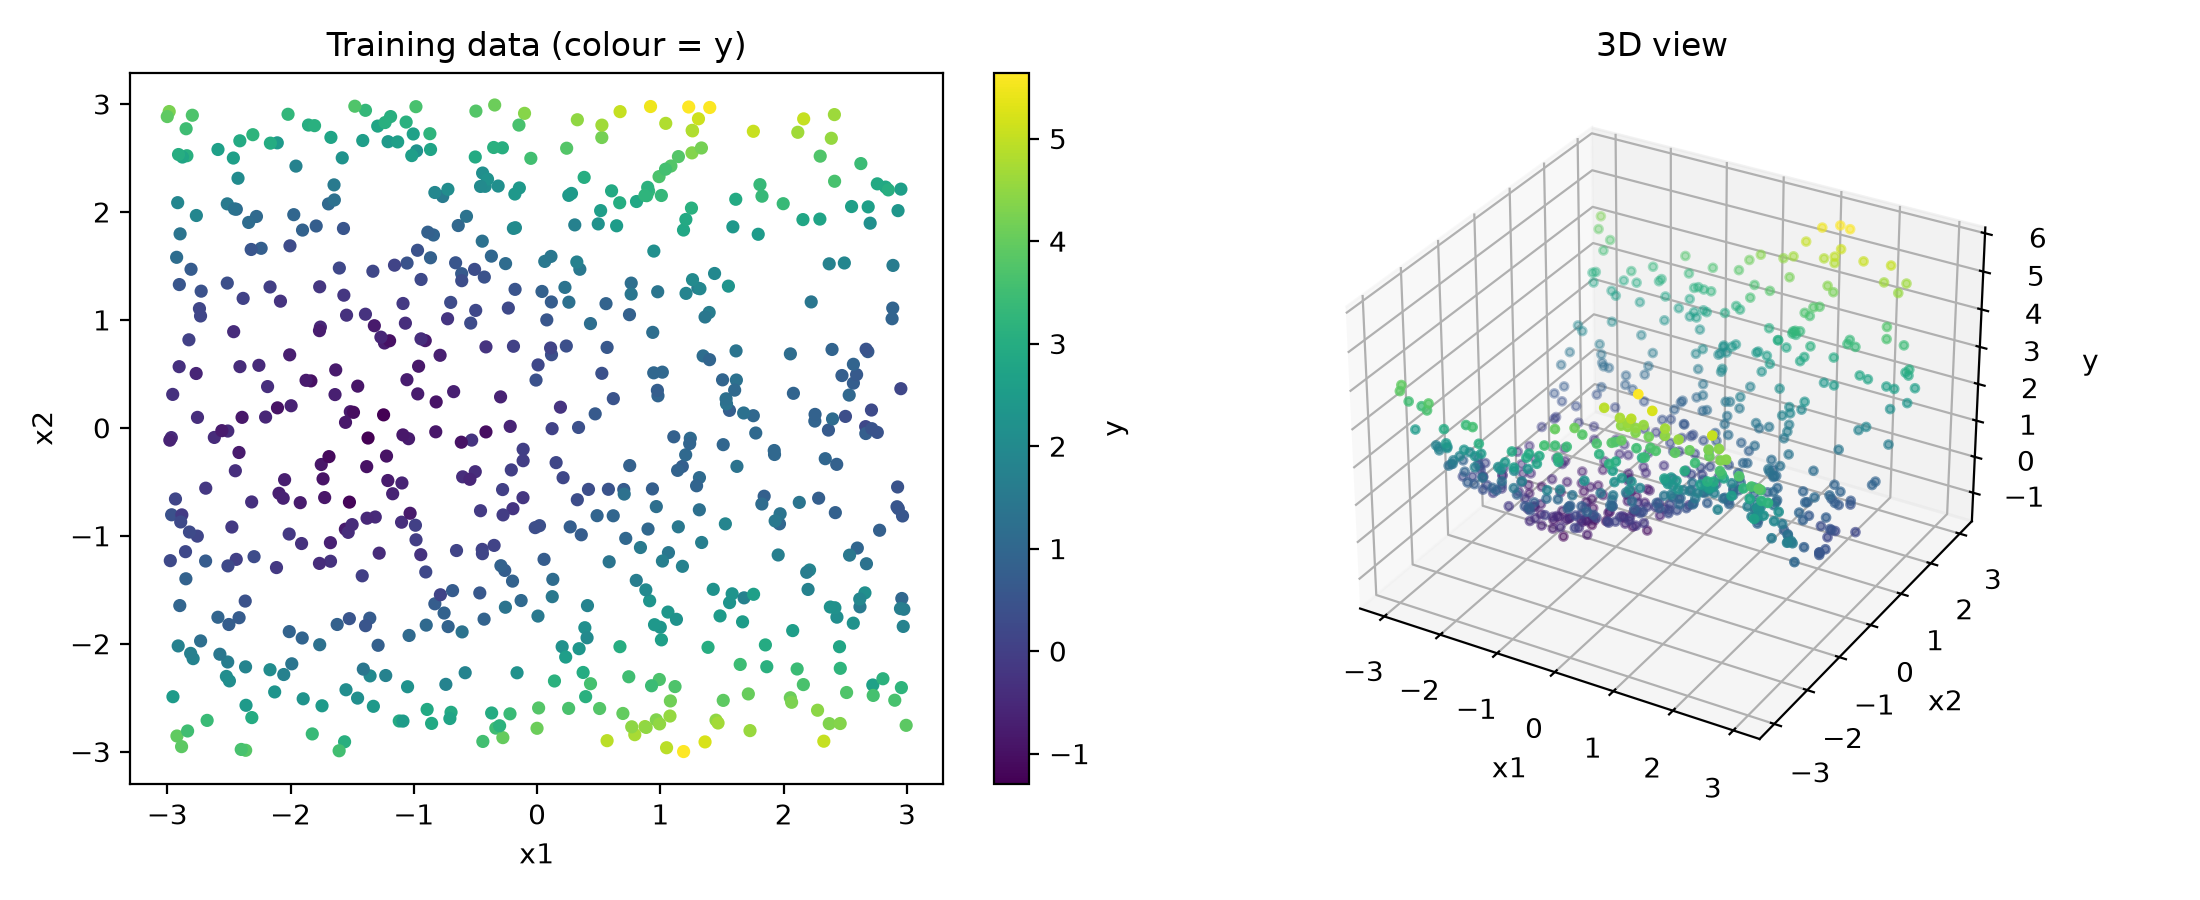
\includegraphics[width=\linewidth]{figs/p3_data.png}\caption{Training data.}\label{fig:data}\end{figure}

  \textbf{(b)} RKS with $D=2000$, $\lambda=10^{-3}$ fixed, sweeping $\sigma$ (the smoothness; $w\sim N(0,I/\sigma^2)$). Small $\sigma$ means high-frequency features: heavily overfit (val MSE 0.98 at $\sigma=0.1$; at $\sigma=0.2$ the validation MSE is about 20; this is not a seed fluke, over 5 random feature draws it ranged from 14 to 44, i.e.\ with $2000>600$ very high-frequency features and tiny $\lambda$ the fit essentially interpolates the noise and extrapolates wildly between training points). Validation MSE decreases to a minimum of 0.0362 at $\sigma=6$ (Figure~\ref{fig:rks}); the best $\sigma=6$. Sweeping $D$ with $\sigma=6$ shows MSE flattening beyond $D\approx50$--$100$ (0.067 at $D=20$, 0.036 at $D=1000$), best $D=1000$ (the values for $D\ge500$ differ only in the fourth decimal). A $\lambda$ sweep at $\sigma=6$ (\texttt{figs/p3\_rks\_lambda.png}) is flat between $10^{-6}$ and $1$ (0.036--0.037), so I kept $\lambda=10^{-3}$. Over 5 random feature draws the final configuration has validation MSE $0.0360$--$0.0364$.
  \begin{figure}[H]\centering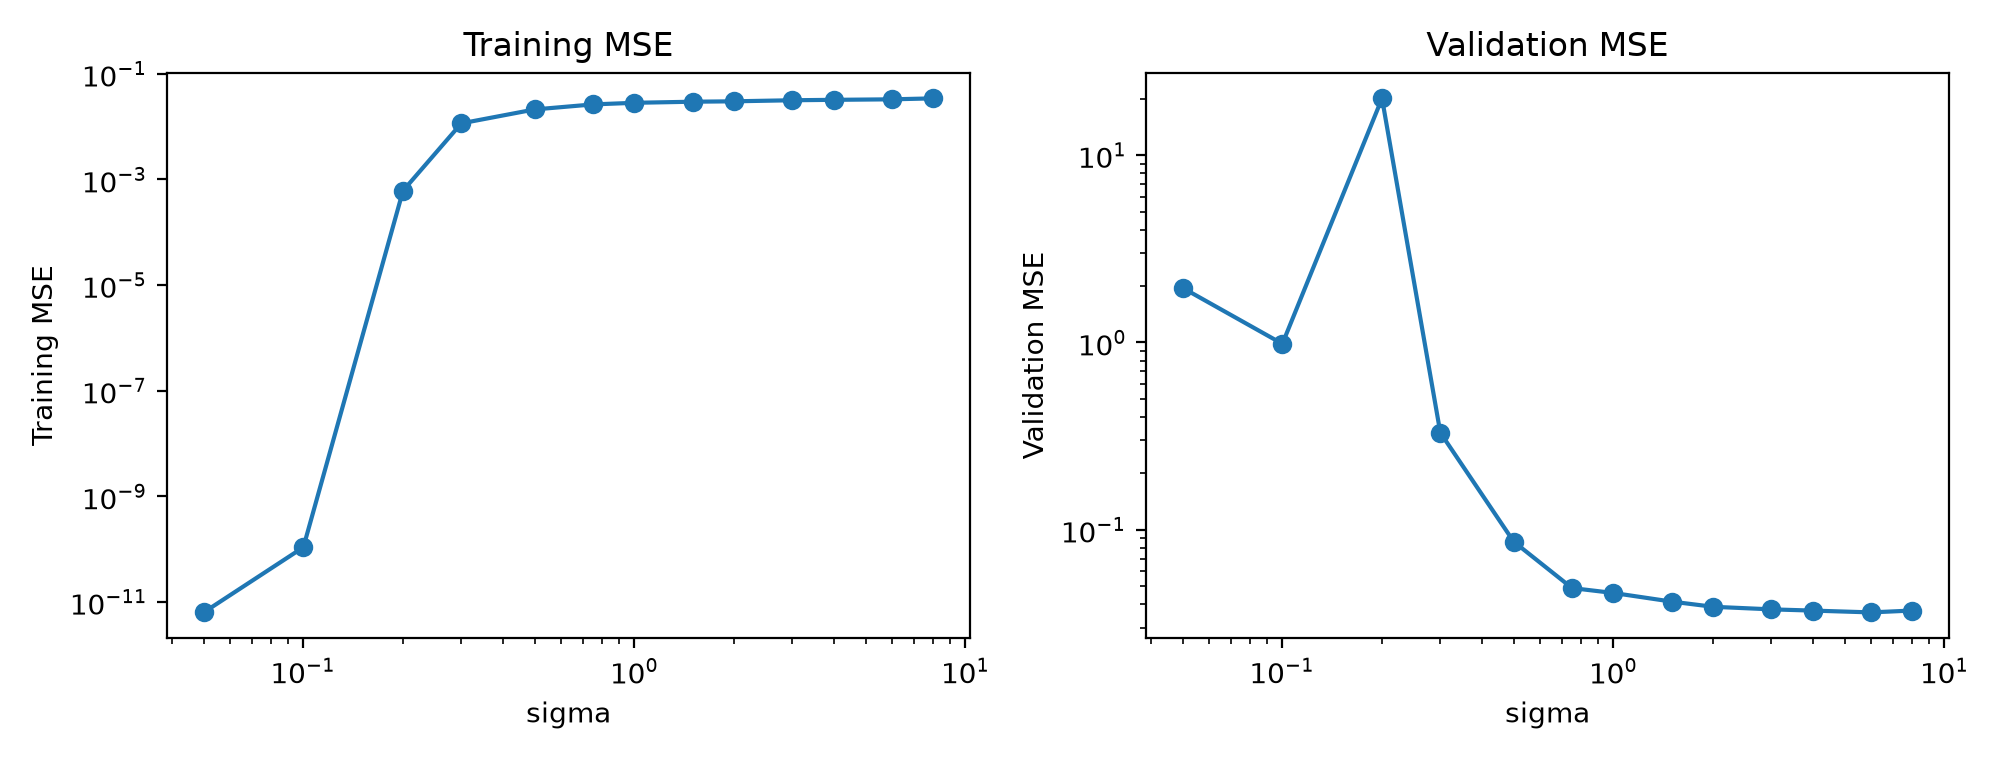
\includegraphics[width=\linewidth]{figs/p3_rks_sigma.png}\caption{RKS: train and validation MSE vs.\ $\sigma$.}\label{fig:rks}\end{figure}

  \textbf{(c)} One-hidden-layer ReLU MLP, Adam, lr $10^{-3}$, batch 128, 300 epochs, sweeping hidden width $\{2,\ldots,512\}$. Validation MSE falls from 0.37 (width 2; width 4 was an unlucky optimization run at 0.94: with other random initializations it gives 0.34 and 0.38) to 0.0390 at width 512, which is the best (Figure~\ref{fig:mlp}). The curve flattens beyond 256 (0.0397), so the larger widths mostly buy small gains.
  \begin{figure}[H]\centering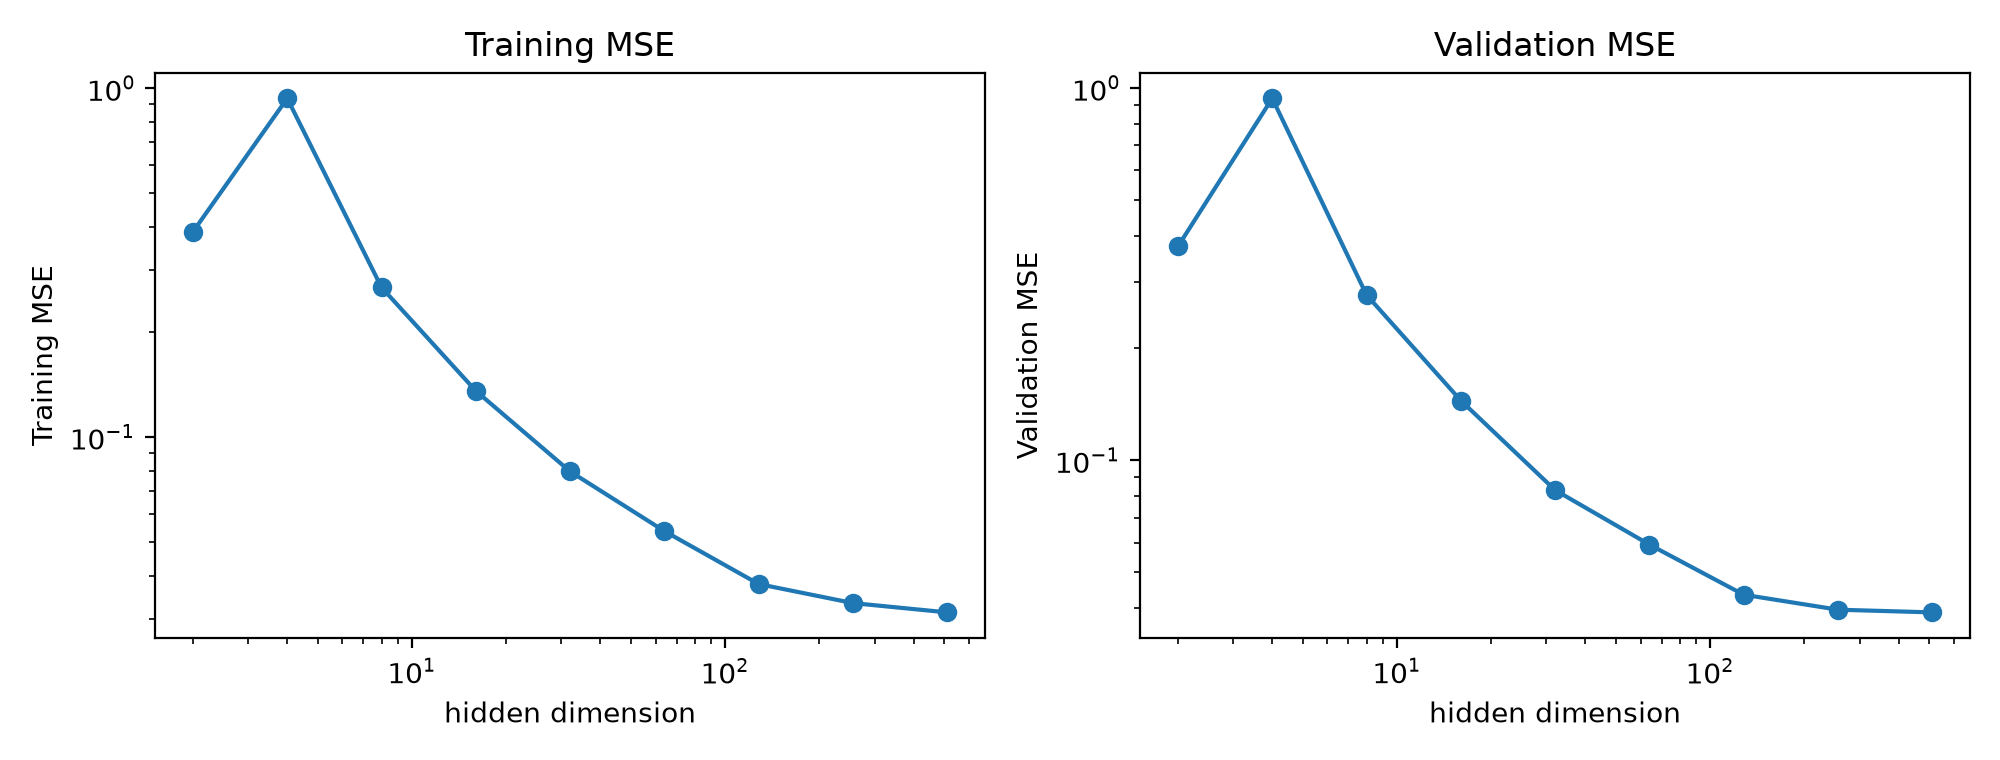
\includegraphics[width=\linewidth]{figs/p3_mlp_hidden.png}\caption{MLP: train and validation MSE vs.\ hidden width.}\label{fig:mlp}\end{figure}

  \textbf{(d)} Refitting with the best hyperparameters:
  \begin{center}
    \begin{tabular}{lcc}
      Model & train MSE & validation MSE \\ \hline
      RKS ($D=1000,\sigma=6,\lambda=10^{-3}$) & 0.0330 & \textbf{0.0360} \\
      MLP (width 512) & 0.0314 & 0.0390 \\
    \end{tabular}
  \end{center}
  (Variance of $y$ on validation is 2.40, so both models explain over 98\% of it.) RKS is better on validation, and it is also much cheaper (a closed-form linear solve vs.\ 300 epochs of SGD). The difference (0.036 vs.\ 0.039) is small in absolute terms and the validation set has only 200 points (and was also used to pick the hyperparameters, so these numbers are slightly optimistic). The ordering is, however, consistent across random seeds: RKS $0.0360$--$0.0364$ over 5 feature draws, MLP $0.0376$--$0.0390$ over 3 initializations. So RKS is modestly but reliably better on this problem, but I would not call it a large effect. RKS, with large $\sigma$, builds in a smoothness prior that matches this smooth target, and its only trained parameters are linear, so it is a convex problem with no optimization noise. The MLP has to learn its features, is a bit more overfit (larger train--val gap), and with ReLU units its surface is piecewise linear, which is a slightly worse match to a smooth function with 600 points. Predictions on \texttt{test.csv} are in \texttt{rks\_test\_predictions.csv} and \texttt{mlp\_test\_predictions.csv} (one per row, same order).

  Figure~\ref{fig:surf} shows the fitted surfaces. Both recover the structure seen in (a): the minimum near $(-1.5,0)$, the rise toward $x_2=\pm3$ with maxima at $x_1\approx1.5$, and the saddle near $(1.5,0)$. The RKS surface is very smooth with nearly elliptical level sets, as expected from a sum of sinusoids at a large length scale. The MLP surface has the same global shape but its contours are slightly wobbly and polygonal, reflecting the piecewise-linear ReLU regions, consistent with a slightly less smooth fit.
  \begin{figure}[H]\centering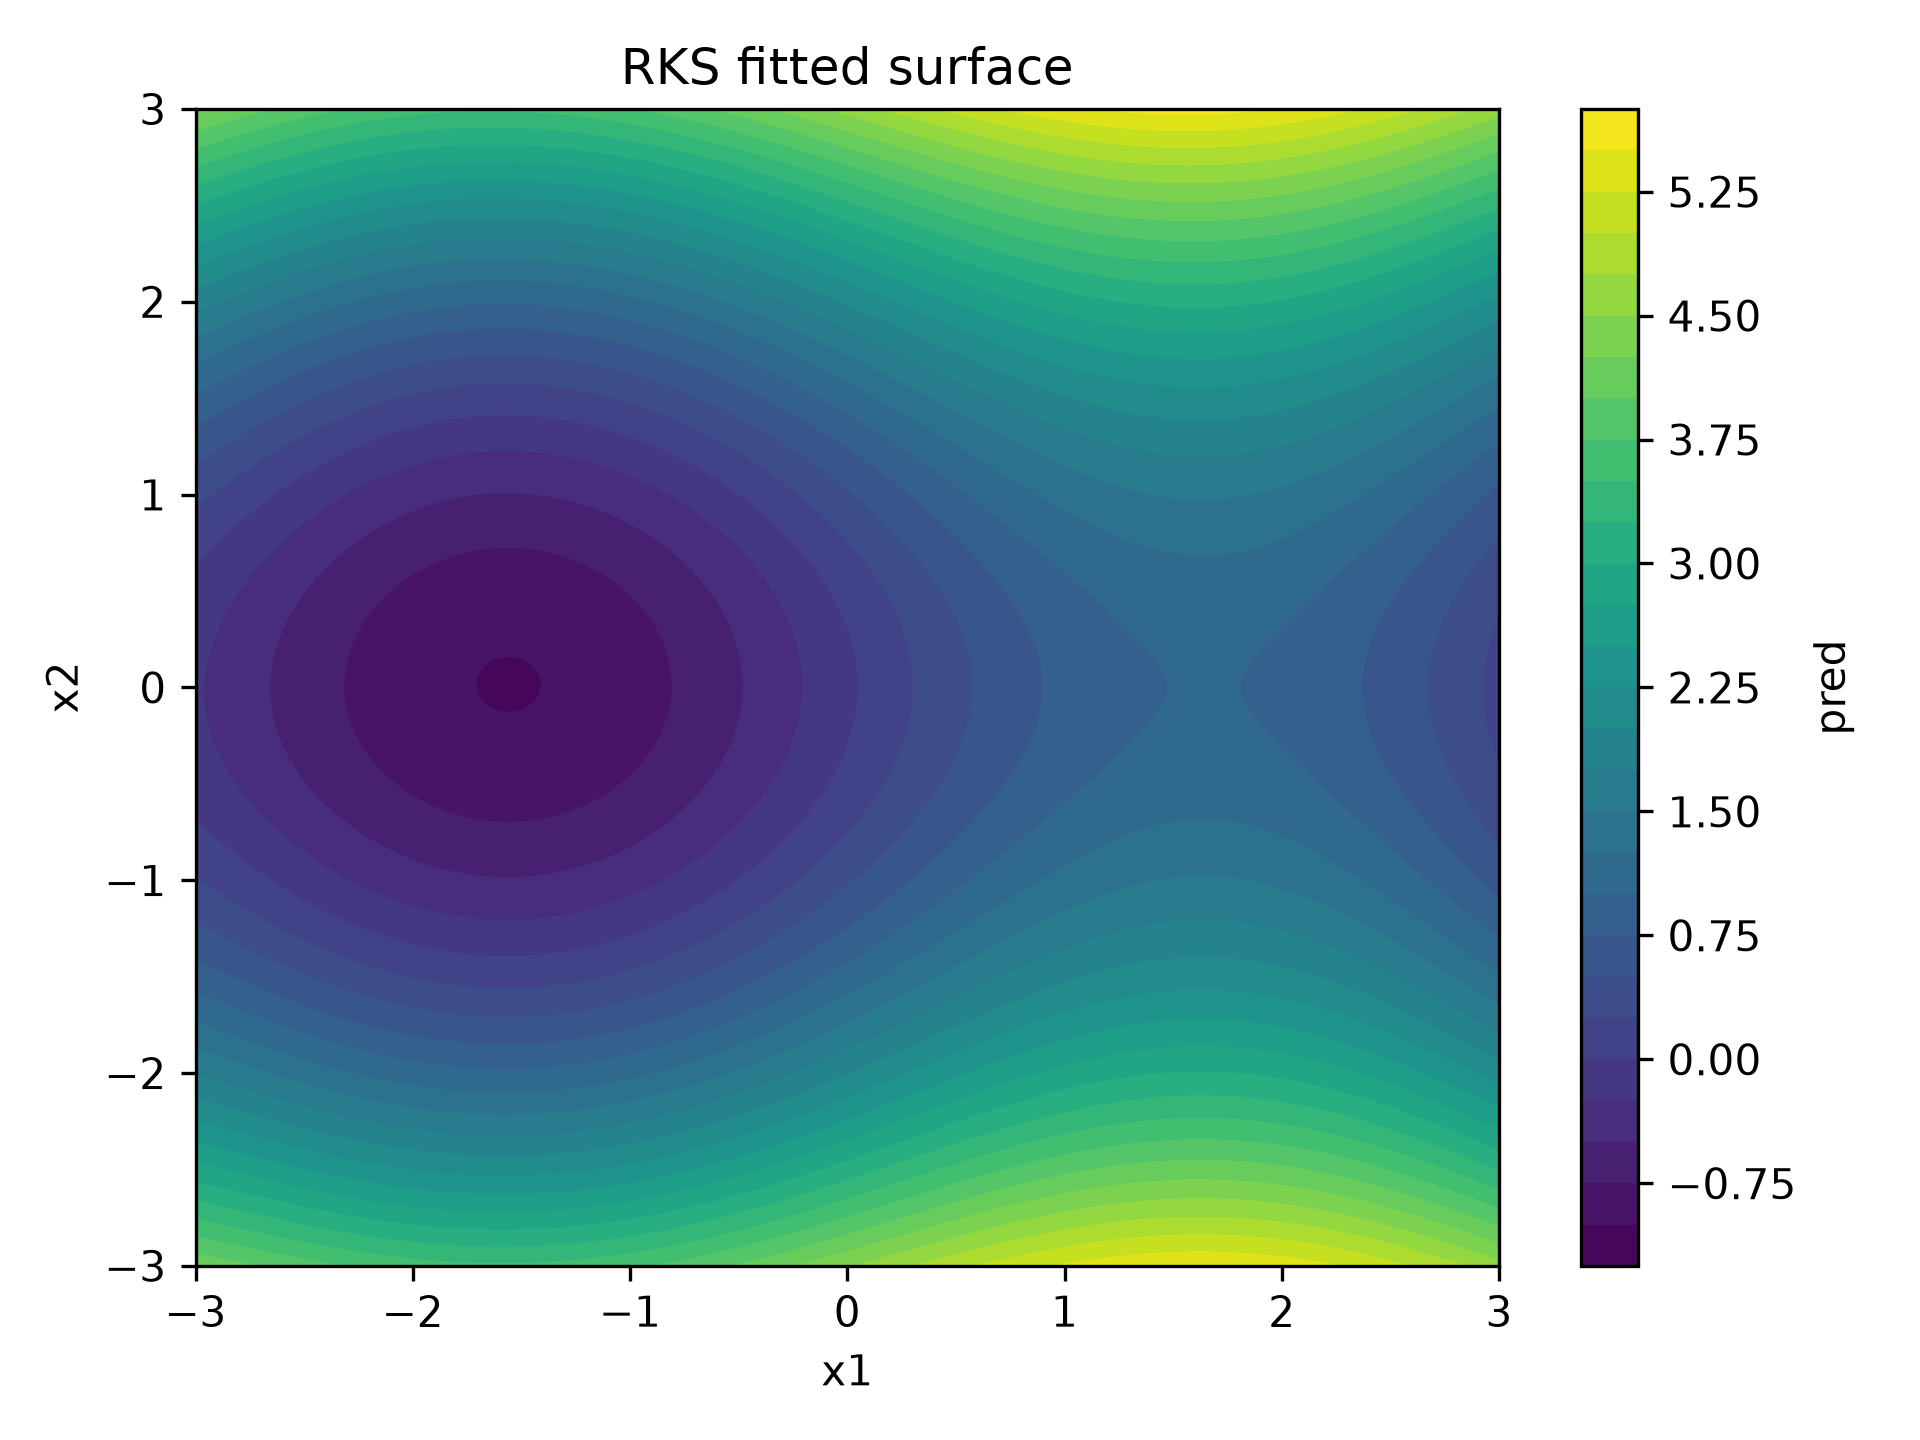
\includegraphics[width=.48\linewidth]{figs/p3_rks_surface.png}\hfill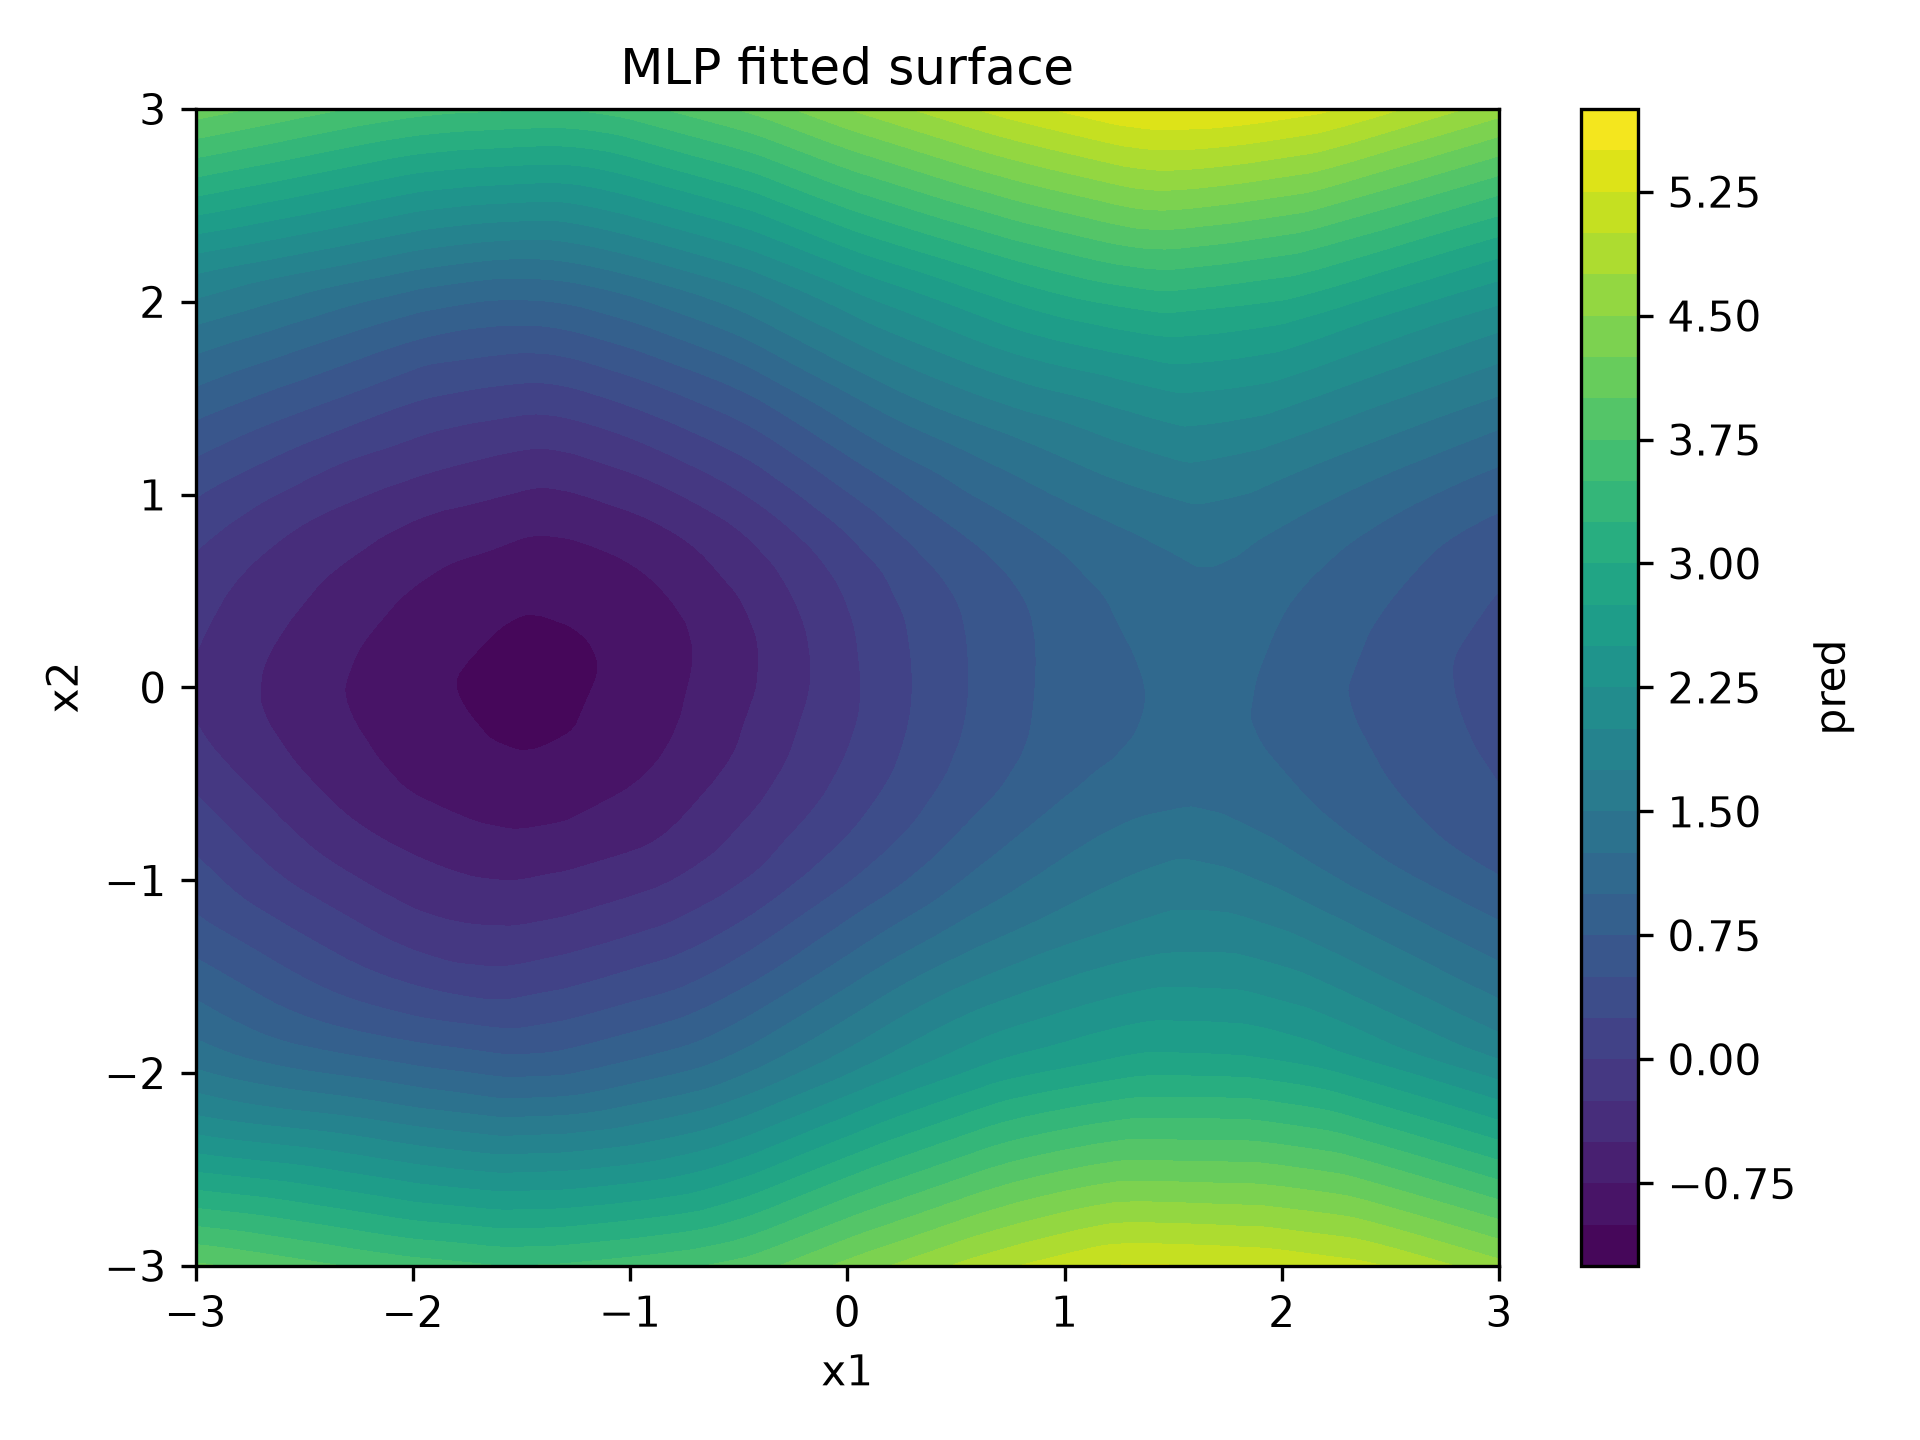
\includegraphics[width=.48\linewidth]{figs/p3_mlp_surface.png}\caption{Fitted surfaces: RKS (left) and MLP (right).}\label{fig:surf}\end{figure}
\end{solution}

\end{document}
